\subsection{Ergebnisse der hand-gefertigten Merkmale} \label{ergebnisse-hc-features-subsec}

Zun{\"a}chst haben wir die Daten mit einer Normalisierungstechnik vorverarbeitet, die bereits im Kapitel \ref{datenerfassung-0} beschrieben wurde.
Entsprechend der ERC haben wir dann den gleitenden Zeitfenster-Segmentierungsansatz (vgl. Kapitel \ref{segmenation-1}) mit den Parametern $T=120$ und $\sigma=30$ verwendet.
Um die optimalen Parameter des SVM-Klassifikators (d.h. Soft-Margin $C$ und Kernelparameter $\gamma$) zu bestimmen, wurde ein Gitter-Suchansatz verwendet.
Es besteht darin, einen Satz m{\"o}glicher Werte f{\"u}r jeden Parameter zu definieren und die Leistungen des Klassifikators f{\"u}r jedes Paar m{\"o}glicher Werte zu testen (d.h. an jedem ``Knoten des Gitters''). \\

\begin{figure}[h]\centering{ \hspace{1cm}
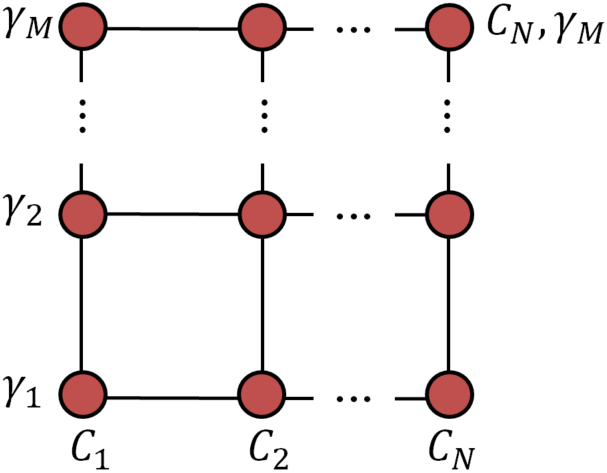
\includegraphics[width=6cm]{Images/grid.png}}
\vspace{0.2cm} \caption[Gitter-Suche]{ Gitter-Suche: Ein definierter Satz m{\"o}glicher Werte f{\"u}r jeden Parameter wird an jedem ``Knoten des Gitters'' getestet. Diese Knoten sind in der Abbildung als rote Punkte markiert. }
\end{figure} 
\vspace{0.5cm}

Die folgenden Werte f{\"u}r $\gamma$ und $C$ wurden getestet:
\begin{center}
${\displaystyle \gamma \in \{0.002; 0.008; 0.03; 0.15; 0.5; 1; 2\}}$ \\
${\displaystyle C \in \{ 0.5; 1; 2; 8; 32; 128; 512 \}}$ \\
\end{center}
\vspace{0.5cm}

Da alle Probanden nicht alle Ziel-Emotionen erlebt bzw. angegeben haben, konnte die Leave-One-Subject-Out Kreuzvalidierung nur bedingt f{\"u}r die Bewertung angewendet werden.
Wir haben daher eine 5-fache Kreuzvalidierung mit entsprechendem F1-Wert verwendet. 

\begin{table}[h]
\center{
\begin{tabular}{|c|c|c|c|c|c|}
\hline
 \textbf{Fold 1} & \textbf{Fold 2} & \textbf{Fold 3} & \textbf{Fold 4} & \textbf{Fold 5} & \textbf{Durchschnitt} \\ \hline
 90.18 & 93.06 & 91.63 & 90.61 & 91.98 & 91.49 \\ \hline
\end{tabular}} \vspace{0.3cm} \caption[Durchschnittlicher F1-Wert]{ Durchschnittlicher F1-Wert in \% f{\"u}r die f{\"u}nf Falten des Datensatzes. }
\end{table}
\vspace{0.5cm}



Die Ergebnisse unserer Experimente zeigen, dass ein solcher Aufbau die Erzielung einer relativ hohen Genauigkeit f{\"u}r die Erkennung der vier Klassen erm{\"o}glicht.
Die Confusion-Matrizen f{\"u}r den handgefertigten Merkmalsansatz unter Verwendung der SVM-Klassifikation ist in der folgenden Tabelle zu finden.

\begin{table}[h]
\center{
\begin{tabular}{|c|c|c|c|c|}
\hline
  & \textbf{Sonstige} & \textbf{Gl{\"u}ck} & \textbf{Frustation} & \textbf{Langeweile} \\ \hline
 \textbf{Sonstige} & \textbf{95.21} & 1.98 & 0.29 & 2.51 \\ \hline
 \textbf{Gl{\"u}ck} & 7.84 & \textbf{90.93} & 0.39 & 0.84 \\ \hline
 \textbf{Frustation} & 8.49 & 2.50 & \textbf{84.14} & 4.87 \\ \hline
 \textbf{Langeweile} & 5.69 & 0.70 & 0.94 & \textbf{92.67} \\ \hline
\end{tabular}} \vspace{0.3cm} \caption[Confusion Matrix]{ Confusion Matrix in \% f{\"u}r die f{\"u}nf Falten des Datensatzes. }
\end{table}